\documentclass{article}

% if you need to pass options to natbib, use, e.g.:
% \PassOptionsToPackage{numbers, compress}{natbib}
% before loading nips_2016
%
% to avoid loading the natbib package, add option nonatbib:
% \usepackage[nonatbib]{nips_2016}

\usepackage[nonatbib, final]{neurips_2020}


% to compile a camera-ready version, add the [final] option, e.g.:
% \usepackage[final]{nips_2016}

\usepackage[utf8]{inputenc} % allow utf-8 input
\usepackage[T1]{fontenc}    % use 8-bit T1 fonts
\usepackage{hyperref}       % hyperlinks
\usepackage{url}            % simple URL typesetting
\usepackage{booktabs}       % professional-quality tables
\usepackage{amsfonts}       % blackboard math symbols
\usepackage{nicefrac}       % compact symbols for 1/2, etc.
\usepackage{microtype}      % microtypography
\usepackage[english]{babel} % for the abstracts
\usepackage{multirow} %for table
\usepackage{makecell} % for tables
\usepackage{float} % positioning
\usepackage{graphicx} % pictures


\title{Speech reconstruction from iEEG data using Deep Learning methods}

\author{
  Donát Ákos Köller \\
  Budapest University of \\ Technology and Economics\\
  \texttt{kollerda@math.bme.hu} \\
  \And
  \textbf{Artúr Vlaszov} \\
  Budapest University of \\ Technology and Economics \\
  \texttt{vlaszova@math.bme.hu} \\
  \And
  \textbf{Emese Vastag} \\
  Budapest University of \\ Technology and Economics \\
  \texttt{evastag@math.bme.hu} \\
}

\begin{document}

\maketitle

\begin{abstract}
  In this project, we attempted to reconstruct speech from intracranial electroencephalography (iEEG) data. The long-term goal of such research is to provide a helping tool for those with communication disorders. We used the SingleWordProductionDutch-iBIDS dataset as a base from which we extracted iEEG features to reconstruct the mel spectrogram and synthesize speech from it. For this task, we used various deep learning methods in order to optimize for one speaker and to create a speaker-independent system. Our results are not useful yet, but we hope in the future we can further improve on them so that they could be applied in real life as well.
\end{abstract}

\begin{center}
{\bfseries\LARGE Agyi jel (iEEG) alapján beszédszintézis deep learning módszerekkel \par}
\end{center}

\begin{kivonat}
  Ebben a projektben beszéd rekonstruálására tettünk kísérletet intrakraniális elektroenkefalográfiás (iEEG) adatokból. Az ilyen kutatások hosszú távú célja, hogy a kommunikációs zavarokkal küzdő emberek számára segédeszközt nyújtsanak. Kiindulásként a SingleWordProductionDutch-iBIDS adathalmazt használtuk, amelyből iEEG jellemzőket vontunk ki, hogy rekonstruáljuk a mel spektrogramot és hogy beszédet szintetizáljunk belőle. Ehhez a feladathoz különböző mélytanulási módszereket használtunk, hogy optimalizáljunk egy beszélőre és hogy egy beszélőfüggetlen rendszert hozzunk létre. Eredményeink még nem használhatóak, de reméljük, hogy a jövőben tovább tudjuk fejleszteni, hogy a valós életben is alkalmazhatóak legyen.
\end{kivonat}

\section{Introduction}

Many people suffer from a condition that prevents them from expressing themselves verbally. For these people, brain-computer interfaces (BCIs) offer viable solutions to help to live with their disabilities. In recent years, many advances were made to use brain signals to synthesize speech and thus provide a real-time communication tool for people with the inability to speak \cite{review1}.

There are numerous ways of capturing brain signals. In our study, we used intracranial electroencephalogram (iEEG) signals, because they provide higher quality than non-invasive methods of recording. The dataset we used consists of iEEG data of 10 subjects, each of them with a different set of electrodes. Our goal during the project was to reproduce the spectral features of speech from the iEEG data. We approached the problem in two ways: we created several models for only one speaker and models which are speaker-independent.

\section{Related works}

Speech decoding and reproduction from brain signals is a highly studied topic and has been the subject of a significant amount of research since the recent advances in machine learning \cite{review2}. The range of applications includes image classification \cite{imgclass}, speech recognition \cite{class1, class2}, speech reconstruction \cite{speechrec} and many other territories as well. While conventional machine learning approaches in these areas can yield great results \cite{svm}, deep learning methods continue to be the most effective tool in achieving outstanding performances.

In the case of speech reconstruction, models which incorporate recurrent neural networks (RNN) \cite{rnn1} and other complex structures such as GAN \cite{sota1} etc. were able to achieve state-of-the-art performance \cite{sota2}. The proposed solutions mainly use data obtained with invasive methods \cite{conv1}, since it is a much more complex task
to effectively reconstruct speech based on non-invasively obtained data.


\section{Data acquisition and preparation}

We used the SingleWordProductionDutch-iBIDS dataset \cite{dataset} which was created with the participation of 10 subjects, each of them suffering from epilepsy. They were implanted with sEEG electrodes as part of the clinical therapy for their epilepsy. They were asked to imagine saying out loud various Dutch words that were shown to them on a monitor, then they were asked to actually say the shown words. The audio, the shown words, and the signals detected by the electrodes were recorded for each participant.

For the one speaker model, we extracted the features we needed based on the same methodology the authors in \cite{dataset} used, meaning we applied IIR bandpass and IIR bandstop filters of order 4 forward and backward, then we averaged the gained Hilbert envelope over 50 ms windows with 10 ms of frameshift. We also stacked 4 non-overlapping, neighboring windows from both the future and the past to each window so that each feature vector will have temporal information coded into them. This way, we obtained the EEG feature vectors, the mel spectrograms of the original audio files, and the corresponding words for each time step.

The data preparation for the speaker-independent model required additional steps. Since the set of electrodes that were used to record the iEEG data was different for each subject, we first needed to set all feature vectors to the same length where each variable represents one of the electrodes in the set. This way, the resulting feature vectors were 4860 dimensional.
Next, two approaches were considered, one of them being reducing the dimensionality of the features for faster modeling, and the other being retaining the original number of features to preserve the 9-time-step sequential nature of the vectors. For the first approach, we used two dimensionality reduction methods: a bottleneck layer of a fine-tuned AutoEncoder and Incremental PCA. The new feature vectors obtained by the two methods were 350 and 250 dimensional respectively. For the second approach, we reshaped the vectors into 9$\times$540 dimensional arrays for them to be used as input for deep learning structures that can decode the sequentiality within the vectors. Scaling was also applied to the data before training.


\section{Modeling}

\subsection{One speaker model}

The reconstruction methodology was the following: we divided the spectrogram into five disjoint parts and then trained the models in five separate iterations to reconstruct each part. In each iteration, four sections were further divided into a training and a validation set (0.8 and 0.2 of the data set). We also standardized the data based on the training set and applied PCA to the feature vectors to reduce their dimensionality which was also fitted on the training set. After this, we trained the model and used it to predict the fifth part. After five iterations the complete spectrogram was reconstructed. Lastly, we used a function to convert it into a proper format and saved it.

We proposed three types of neural network models for the one-speaker model:
\begin{itemize}
    \item Fully Connected Dense Neural Network (FC-DNN) with a bottleneck layer
    \item Normal FC-DNN
    \item Bidirectional Gated Recurrent Unit (BiGRU) based network
\end{itemize}

For the first two models, the size of the input layer was set to 200. The Bottleneck model was constructed with six dense layers, the last one being the size of the output, and the first five having sizes that first decrease, then grow. The Normal FC-DNN model has four dense layers which decrease in size gradually, down to the last being once again the size of the output.

The BiGRU model has a different input layer, in this case, the shape is fixed to (9, 127). The model has two Bidirectional GRU layers, a flattening layer and a dense layer as an output.


\subsection{Speaker-independent model}

For both the lower dimensional and the higher dimensional data, we split the whole dataset into train, validation and test set in a 60-20-20 ratio. In order to make sure that each set contains approximately equal amount of data from each subject while also ensuring the diversity of the feature vectors, we split the data of each subject into 5 approximately equal, disjoint parts, then iteratively, we changed which of the 5 parts would be in which set. With 10 participants, this meant 2 full cycles of iterations after which the train set had 179011, the validation set had 59672 and the test set had 59672 elements. We did the same procedure with the mel spectrograms as well.

We trained a simple fully-connected neural network on both the 350 and the 250-dimensional data. In both cases, we measured the RMSE and the mean correlation with the original spectrograms. The results achieved with the 250-dimensional data were more impressive so we only optimized the hyperparameters for this model. The final model consists of 5 dense layers using dropout as well.

For the 9$\times$540 dimensional features, we built two types of models, one of them being a BiGRU-based network and the other being a convolutional neural network. The BiGRU network consists of 2 recurrent layers with dropout, a fully connected dense layer with dropout, and an output layer. The convolutional network was constructed with two 1D convolution layers with a dropout layer between them, followed by a 1D max pooling layer, a flattening layer, and the output layer.

\subsection{Optimization}

Aside from using Adam optimizer and mean squared error as loss, hyperparameter optimization was also implemented for every network structure in both the one-speaker model and the speaker-independent model. We used Keras-tuner hyperband optimization. We used different batch sizes, training epochs, and early stopping limits depending on the models and networks, the values varied between 64-512, 80-100, and 8-25 respectively. 

The baseline models showed decent results, so their layer structure remained the same. The sizes of the layers, the learning rate, and the dropout rates were optimized. For each hyperparameter, we created sets of values that were close to the original value. We usually let the tuner pick from four, five, or slightly more options.

For the one-speaker model, after defining the model structure, the reconstruction of the mel spectrogram was done in five folds. In each fold, we initialized and ran the tuner to achieve the best results.

For the speaker-independent model, since the amount of training data was vastly larger than in the one-speaker model, we had to limit the number of maximum training epochs and hyperparameter options for the optimizations to finish within a reasonable amount of time.

\section{Evaluation and results}

We used three metrics to evaluate the performances of the models: RMSE, mean Pearson correlation, and MCD (Mel Cepstral Distortion) which is an objective measure for evaluating synthetic voices. For the one-speaker model, the RMSE was averaged out across the reconstruction folds, while for the speaker-independent system, the MCD was averaged out on the ten disjoint parts of the spectrogram which came from different subjects. Table \ref{tab:results} shows the performances of the optimized models. Although our models got relatively good MCD and correlation scores, hearing the reconstructed audio files proves that the quality of the synthesized speech is low, and the words are not understandable.

\begin{table}[ht]
  \caption{Results of the different models with different metrics.}
  \label{tab:results}
  \centering
  \begin{tabular}{llccc}
    \toprule
    &&\multicolumn{3}{c}{Metrics} \\
    \cmidrule{3-5}
    Model type & Network   & RMSE    & Pearson corr. & MCD \\
    \midrule
   \multirow{3}{*}{One-speaker model}& Bottleneck & {\bf 1.5783} & {\bf 0.5670} & 4.7027     \\
    & FC-DNN & 1.5895 & 0.5661 & 7.8219  \\
    & BiGRU   & 1.6071 & 0.5627& {\bf 4.3637}  \\
    \midrule
    \multirow{3}{*}{\makecell{Speaker-independent \\ model}} & FC-DNN & 1.4876 & 0.7329 & {\bf 1.2362}\\
    & BiGRU & {\bf 1.4536} & {\bf 0.7356} & 1.3598 \\
    & Convolutional & 1.4737 & 0.7273 & 1.6827 \\ 
    \bottomrule
  \end{tabular}
\end{table}

As an example of our results with the one-speaker model, Figure \ref{fig:one_speaker} shows a comparison between the original and the reconstructed spectrogram with the BiGRU model.

\begin{figure}
    \centering
    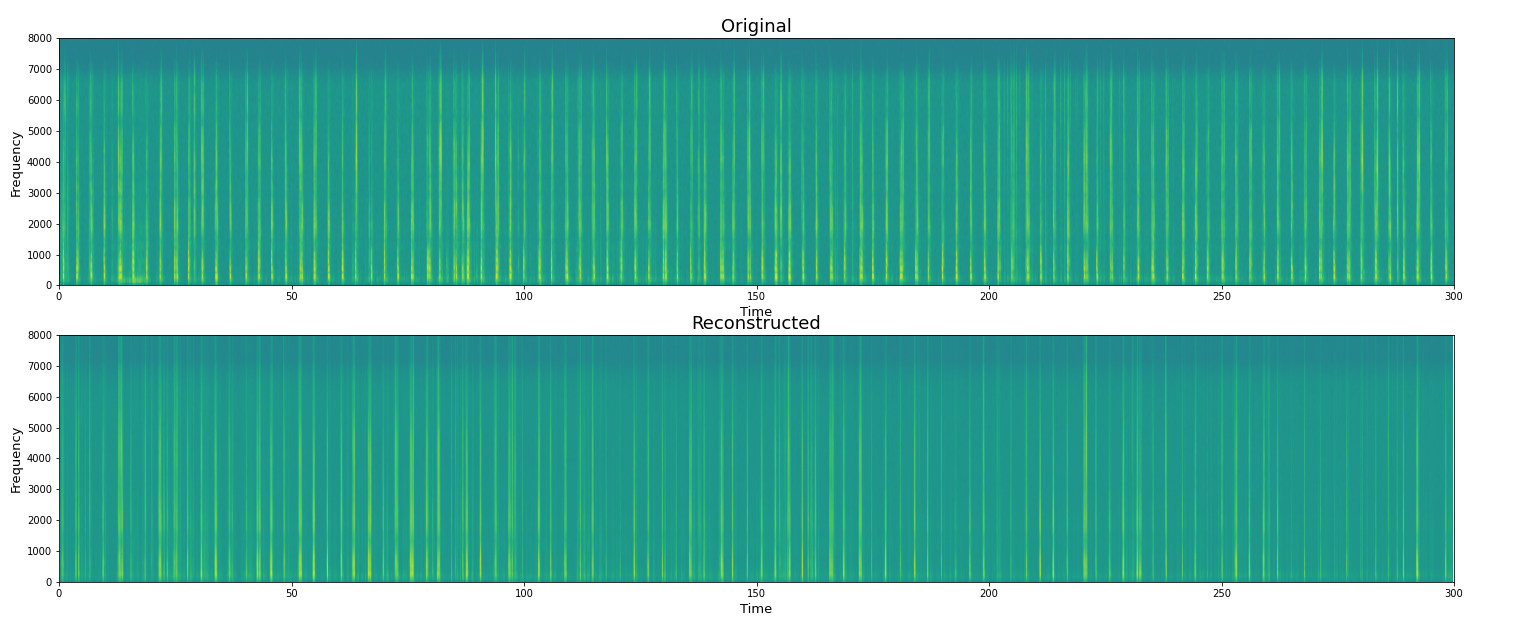
\includegraphics[width=\textwidth]{one_speaker.png}
    \caption{Results of the one-speaker BiGRU model.}
    \label{fig:one_speaker}
\end{figure}

On Figure \ref{fig:indep} we show the results of the speaker-independent model with the fully-connected neural network, which yielded the best MCD score.

\begin{figure}
    \centering
    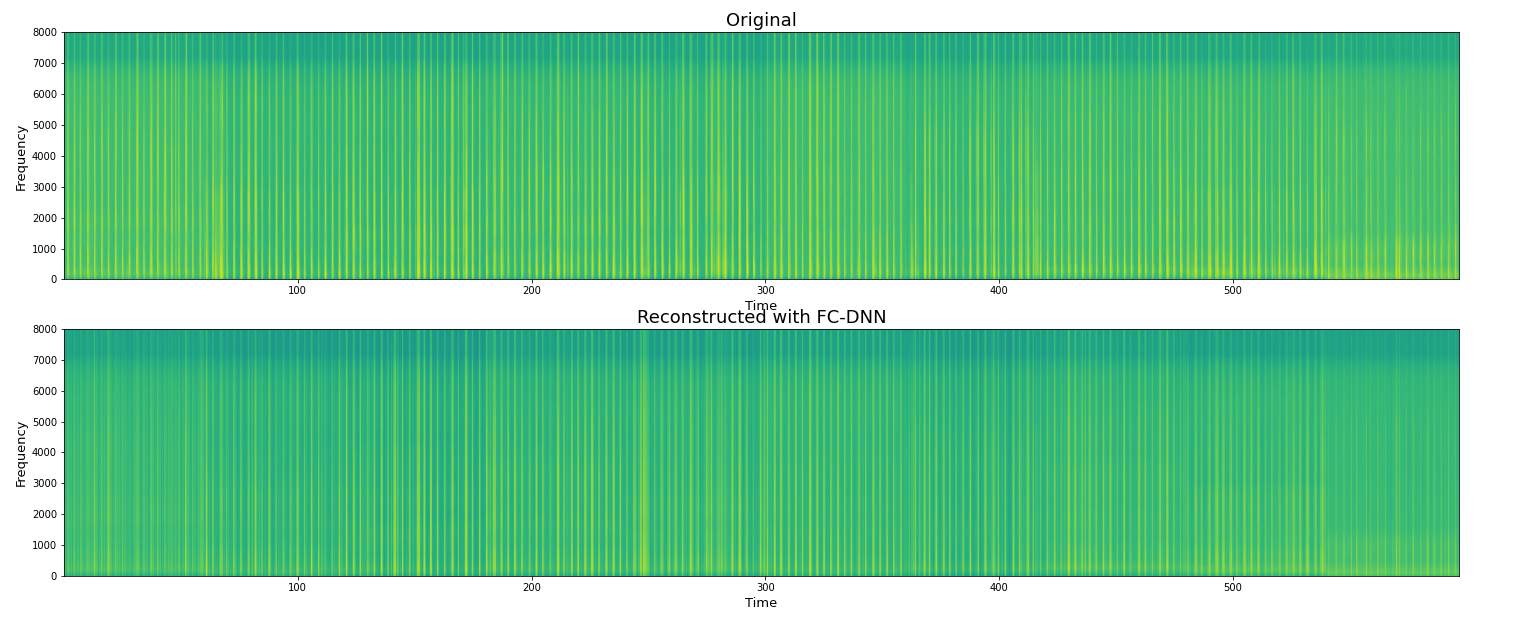
\includegraphics[width=\textwidth]{speak_indep.png}
    \caption{Results of the speaker-independent fully-connected model.}
    \label{fig:indep}
\end{figure}


\section{Conclusions, future plans}
In this project, we aimed to synthesize speech from iEEG data using various deep neural networks. We implemented numerous data preparation methods and models to achieve better results in both one-speaker modeling and speaker-independent systems.

By analyzing the reconstructed spectrograms and comparing them to the original ones we can conclude that the models have the ability to learn certain patterns and to recreate them, but the more complex ones are usually shifted. This means that the work in this direction has great perspectives.

The hyperparameter optimization greatly improved the results of the different models and in most cases resulted in better MCD scores, although the Pearson correlation sometimes did not increase.
Although some of the results seem fairly good, they are far from being optimal. According to our experiences, even better results can be achieved with wider optimisation space and more complex, combined neural networks.

Our further goals include testing the network structures that have proven to be best for the one-speaker model on other participants, and trying out different vocoder models for speech synthesis, such as WaveGlow\cite{waveglow} or HifiGAN\cite{hifigan}. 

\section{Acknowledgements}

We would like to express our gratitude to our supervisor, Tamás Gábor Csapó who provided us with lots of useful advice and insights about the topic and the modeling.


\begin{thebibliography}{9}

\small

\bibitem{review1} Panachakel, J. T., \& Ramakrishnan, A. G. (2021). Decoding Covert Speech From EEG-A Comprehensive Review. Frontiers in neuroscience, 15, 642251. https://doi.org/10.3389/fnins.2021.642251

\bibitem{review2} Lopez-Bernal, D., Balderas, D., Ponce, P., Molina, A. (2022). A State-of-the-Art Review of EEG-Based Imagined Speech Decoding. {\it Frontiers in human neuroscience, 16}, 867281. https://doi.org/10.3389/fnhum.2022.867281

\bibitem{class1} Chengaiyan, S.,  Retnapandian, A. S., \& Anandan, K. (2020). Identification of vowels in consonant-vowel-consonant words from speech imagery based EEG signals. {\it Cognitive neurodynamics, 14}(1), 1–19. https://doi.org/10.1007/s11571-019-09558-5

\bibitem{class2} Sarmiento, L. C., Villamizar, S., López, O.,  Collazos, A. C.,  Sarmiento, J., \&  Rodríguez, J. B. (2021). Recognition of EEG Signals from Imagined Vowels Using Deep Learning Methods. {\it Sensors (Basel, Switzerland), 21}(19), 6503. https://doi.org/10.3390/s21196503

\bibitem{rnn1} Al-Radhi, M. S., Csapó, T. G., \&  Németh, G. (2019). RNN-based speech synthesis using a continuous sinusoidal model. {\it CoRR, abs/1904.06075.} Retrieved from http://arxiv.org/abs/1904.06075

\bibitem{rnn2} Saha, P., \& Fels, S. (2019). Hierarchical Deep Feature Learning for Decoding Imagined Speech from EEG. {\it Proceedings of the AAAI Conference on Artificial Intelligence, 33}(01), 10019-10020. https://doi.org/10.1609/aaai.v33i01.330110019

\bibitem{dataset} Verwoert, M., Ottenhoff, M.C., Goulis, S. et al. (2022). Dataset of Speech Production in intracranial Electroencephalography. {\it Sci Data} {\bf 9}, 434. https://doi.org/10.1038/s41597-022-01542-9

\bibitem{conv1} Angrick, M., Ottenhoff, M., Goulis, S., Colon, A., Wagner, L., Krusienski, D., Kubben, P., Schultz, T., \& Herff, C. (2021). Speech Synthesis from Stereotactic EEG using an Electrode Shaft Dependent Multi-Input Convolutional Neural Network Approach. {\it 2021 43rd Annual International Conference of the IEEE Engineering in Medicine \& Biology Society (EMBC)} (pp. 6045-6048). doi:10.1109/EMBC46164.2021.9629711

\bibitem{sota1} Krishna, G., Tran, C., Carnahan, M., \& Tewfik, A. H. (2021). Advancing Speech Synthesis using EEG. {\it 2021 10th International IEEE/EMBS Conference on Neural Engineering (NER)}, 199–204. doi:10.1109/NER49283.2021.9441306

\bibitem{sota2}  Krishna, G., Han, Y., Tran, C., Carnahan, M., \& Tewfik, A. H. (2019). State-of-the-art Speech Recognition using EEG and Towards Decoding of Speech Spectrum From EEG. {\it ArXiv E-Prints}, arXiv:1908.05743. Retrieved from http://arxiv.org/abs/1908.05743

\bibitem{sota3}  Krishna, G., Tran, C., Carnahan, M., \& Tewfik, A. (2019). Advancing Speech Recognition With No Speech Or With Noisy Speech. {\it 2019 27th European Signal Processing Conference (EUSIPCO)}, 1–5. doi:10.23919/EUSIPCO.2019.8902943

\bibitem{imgclass} Zhang, K., Robinson, N., Lee, S. W., \& Guan, C. (2021). Adaptive transfer learning for EEG motor imagery classification with deep Convolutional Neural Network. {\it Neural networks : the official journal of the International Neural Network Society, 136,} 1–10.

\bibitem{waveglow} Prenger, R., Valle, R., \& Catanzaro, B. (2018). WaveGlow: A Flow-based Generative Network for Speech Synthesis. {\it ArXiv E-Prints}, arXiv:1811.00002. Retrieved from http://arxiv.org/abs/1811.00002

\bibitem{hifigan} Kong, J., Kim, J., \& Bae, J. (2020). HiFi-GAN: Generative Adversarial Networks for Efficient and High Fidelity Speech Synthesis. {\it ArXiv E-Prints}, arXiv:2010.05646. Retrieved from http://arxiv.org/abs/2010.05646

\bibitem{svm} DaSalla, C. S., Kambara, H., Sato, M., \& Koike, Y. (2009). Single-trial classification of vowel speech imagery using common spatial patterns. {\it Neural Networks, 22}(9), 1334–1339. doi:10.1016/j.neunet.2009.05.008

\bibitem{speechrec} Wu, H., \& Chen, F. (2020). A Temporal Envelope-based Speech Reconstruction Approach with EEG Signals during Speech Imagery. {\it 2020 Asia-Pacific Signal and Information Processing Association Annual Summit and Conference (APSIPA ASC)}, 894–899.



\end{thebibliography}

\end{document}
